\documentclass{beamer}

\usepackage{beamerthemesplit}
\usepackage{amsmath}
\usepackage{amsfonts}
\usepackage{amssymb}
\usepackage{qtree}
\usepackage{cancel}
\usepackage{tkz-graph}
\usepackage{bussproofs}
%\usepackage[pdftex]{graphicx}

\makeatletter
\newcommand{\reallytiny}{\@setfontsize{\srcsize}{2pt}{2pt}}
\makeatother

\mode<presentation>
{
  \usetheme{metropolis}
  % or ...

  %\setbeamercovered{transparent}
  % or whatever (possibly just delete it)
}

\usepackage[english]{babel}
% or whatever

\usepackage[latin1]{inputenc}
% or whatever

\usepackage{times}
\usepackage[T1]{fontenc}

\title{Inferential Approach to Mining Surprising Patterns in
  Hypergraphs}

\author{Nil Geisweiller, Ben Goertzel}

\institute[SingularityNET OpenCog Foundations] % (optional, but mostly needed)
{
  \begin{center}
    
\includegraphics[scale=0.5]{images/snet_oc.png}
  \end{center}
}

\date[AGI-19] % (optional, should be abbreviation of conference name)
{AGI-19, Shenzhen}

%\newcommand{\AND}{\textit{AND}}
%\newcommand{\OR}{\textit{OR}}
%\newcommand{\NOT}{\textit{NOT}}
\newcommand{\AND}{\land}
\newcommand{\OR}{\lor}
\newcommand{\NOT}{\lnot}

\begin{document}

\frame
{
%%%%%%%%%%%%
%% Speech %%
%%%%%%%%%%%%

%% This work starts with the motivation of reframing learning as an
%% explicit form of reasoning.

%% We claim that by doing that, reframing learning as reasoning you
%% gain more transparency and as a result you make it much easier to
%% enable meta-learning at all levels.

%% Here in particular we are gonna focus on mining suprising patterns.

%% All the work I'm gonna present here is implemented with the OpenCog
%% framework, and it is sponsored by SingularityNET.

%%%%%%%%%%%%%
%% ~Speech %%
%%%%%%%%%%%%%

  \maketitle
}

\begin{frame}
  \frametitle{Reframing \alert{learning as reasoning}}

%%%%%%%%%%%%
%% Speech %%
%%%%%%%%%%%%

%% OK, so what does reframing learning as reasoning mean?

%% What it means is, just think of any learning task, such as learning
%% how to recognize faces, which is translated as a task of proving a
%% certain theorem or a collection of theorems in a certain theory.

%%%%%%%%%%%%%
%% ~Speech %%
%%%%%%%%%%%%%

  \begin{columns}

    \column{2in}
    %% \begin{center}Learning\end{center}
    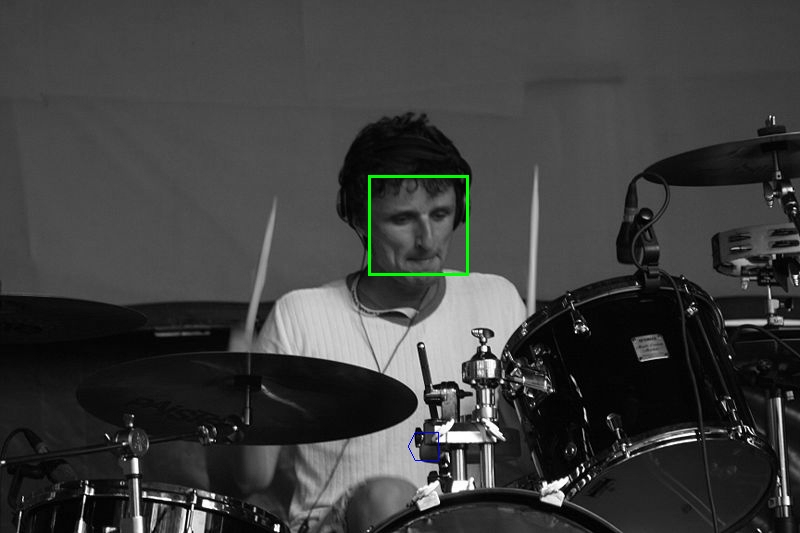
\includegraphics[scale=0.15]{images/800px-Cool_Kids_of_Death_Off_Festival_p_146-face_selected.jpg}

    \column{1in}
    $$ \Rightarrow $$

    \column{1in}
    %% \begin{center}Reasoning\end{center}
    $$ \mathcal{T} \vdash \mathcal{F} $$

  \end{columns}

\end{frame}

\begin{frame}
  \frametitle{Reframing \alert{mining surprising patterns as
      reasoning}}

%%%%%%%%%%%%
%% Speech %%
%%%%%%%%%%%%

%% More specifically we're gonna show how to do that for 2 problems

%% 1. the problem of finding frequent patterns in a database

%% 2. and the problem of assessing their surprisingness

%% To give you a broader picture. The reason we are interested in
%% these 2 problems, is because they are part of a greater
%% meta-learning scheme that I'm gonna present right now, that can be
%% called "Inference Control Meta-learning".

%%%%%%%%%%%%%
%% ~Speech %%
%%%%%%%%%%%%%

  \begin{enumerate}
  \item Learning \alert{frequent} patterns
  \item Assessing their \alert{surprisingness}
  \end{enumerate}

\end{frame}

\begin{frame}
  \frametitle{Inference Control Meta-learning}

%%%%%%%%%%%%
%% Speech %%
%%%%%%%%%%%%

%% As you probably already know the problem of reasoning is that it
%% rather inefficient in general, there is a combinatorial explosion
%% due to the number of rules and premises that can be chosen from to
%% build an inference. The complexity is basically growing exponential
%% with the size of the proof.

%% So it's important to be able to learn how to reason
%% efficiently. But once you reframe learning as reasoning, then it
%% becomes the problem of how to reason to reason efficiently, and
%% that creates a very direct feedback loop in your system.

%% I'm gonna present very briefly the system we have in place to do
%% that with opencog.

%% We have a rewriting system that we call the unified rule engine,
%% that can be used to implement any logical system, what it does is
%% that essentially evolves inference trees, either in a forward
%% fashion, from premises to conclusions, from theory to theorems, or
%% in a backward fashion, from conclusions to premises, from theorems
%% to theory.

%% Now the interesting thing about it is that it can use control rules
%% to decide how to select premises or conclusion and rules to
%% construct these inference trees, and so the idea is that if we can
%% learn the right control rules we can speed up reasoning. And that
%% is where pattern mining comes into place here, as a simple though
%% efficient way to kick start such feedback loop.

%% There is BTW another component of OpenCog called ECAN, that stands
%% for Economic Attention Allocation Networks, that is also designed
%% to speed up reasoning, that I'm letting aside here.

%%%%%%%%%%%%%
%% ~Speech %%
%%%%%%%%%%%%%

  Learning how to \alert {reason efficiently}.

  \begin{itemize}
  \item<+-> Unified Rule Engine
    \begin{itemize}
    \item Evolves Inference Trees
      TODO: add pic
    \item \alert{Control Rules} to select premises and rules
    \end{itemize}
  \item<+-> Learn Control Rules for efficient reasoning
    TODO: diagram with learning control rules controlling inference.
  \end{itemize}
\end{frame}

\begin{frame}
  \frametitle{Mining Frequent Patterns}

%% A specialization is a pattern that encompasses less instances than
%% its abstraction. For instance the pattern ``black cat'' is a
%% specialization of its abstraction ``cat''.

  Brute force algorithm:
  \begin{itemize}
  \item $S$: minimum support
  \item $P$, $Q$: patterns
  \item $\mathcal{C}$: pattern pool
  \item $\mathcal{D}$: database
  \end{itemize}
  
  \begin{enumerate}
  \item Select $P$ from $\mathcal{C}$
  \item Select \emph{specialization} $Q$ of $P$ such that $S \leq
    \texttt{support}(Q, \mathcal{D})$
  \item Add $Q$ to $\mathcal{C}$
  \item Repeat
  \end{enumerate}

\end{frame}

\begin{frame}
  \frametitle{Mining Frequent Patterns as Reasoning}

  \begin{prooftree}
    \AxiomC{$S \leq \texttt{support}(Q, \mathcal{D})$}
    \AxiomC{$\texttt{spec}(Q, P)$}
    \RightLabel{(AP)}
    \BinaryInfC{$S \leq \texttt{support}(P, \mathcal{D})$}
  \end{prooftree}

  TODO: make mini inference tree expansion example.

\end{frame}

\begin{frame}
  \frametitle{Mining Surprising Patterns}

%% First we need to define what is surprisingness, we define
%% surprisingness as what is contrary to expectation, it is the
%% unexpected.

%% So whatever deviates from expectation is surprising and the more it
%% deviates, the more surprising it is.

%% So the working definition we gonna take is gonna be the distance
%% between empirical probability of a event and the probability
%% estimate of that event. However probabilities are generally unknown
%% we only ever have approximations, even for the empirical
%% probability, so instead of considering individual probabilities we
%% are gonna consider envelopes of probabilities to capture the
%% uncertainties, both of the empirical probability which is gonna
%% exist because we always a finite number of observations, and of the
%% probability estimate because we typically have a multi-world type
%% of understanding at any point in time, so we have even more
%% uncertainty there.

%% OK, so why does that matter, because what is surprising is
%% typically gonna carry more information gain, it's hard to predict
%% and so it is hard to reconstruct. So we really need to pay
%% attention to it, either to remember it, or to remodel our
%% understanding, etc.

%% But once something has been surprising, if the system has done a
%% proper job at analyzing it, it should no longer be surprising, so
%% we need a dynamic measure of surprisingness. The way we do that, is
%% to allow the full spectrum of reasoning to infer the probability
%% estimate rather than a hard wired scheme based on some predefined
%% assumptions.

%% But typically we have something more spread out, often multi modal
%% where each mode corresponds to set of hypothesis.
  
  \textcolor{blue}{Definition}
  \begin{center}\emph{surprise}: \alert{contrary to expectation}\end{center}

  \begin{center}
    \only<1>{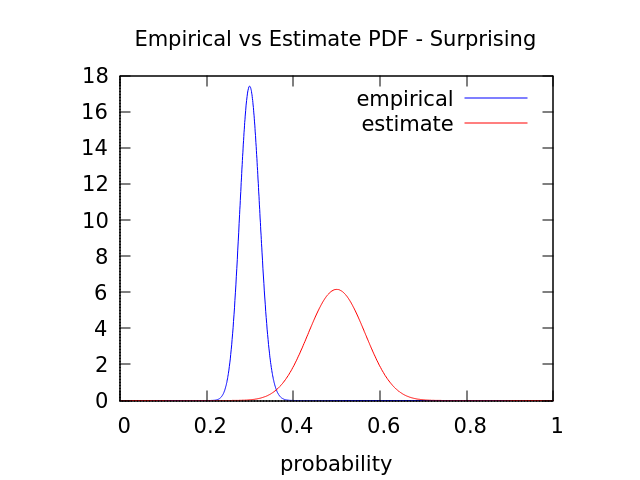
\includegraphics[scale=0.85]{images/surprising.png}}
    \only<2>{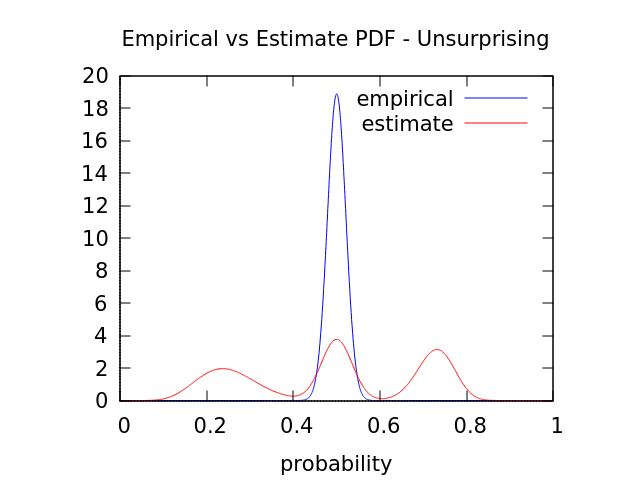
\includegraphics[scale=0.85]{images/unsurprising.png}}
  \end{center}

\end{frame}

\begin{frame}
  \frametitle{Mining Surprising Patterns as Reasoning}
  TODO
\end{frame}

\begin{frame}
  \frametitle{Examples}
\end{frame}

\end{document}
